\documentclass[a4paper,12pt]{report}

% Espacement entre les texte 
\usepackage{setspace}
\usepackage[a4paper, margin=1in]{geometry}

% Encodage et langue
\usepackage[utf8]{inputenc}
\usepackage[T1]{fontenc}
\usepackage[numbers]{natbib}
\usepackage[french]{babel}

% Mise en page
\usepackage{geometry}
\geometry{a4paper, margin=2.5cm}

% Packages utiles
\usepackage{graphicx}
\usepackage{amsmath, amssymb}
\usepackage{hyperref}
\usepackage{float}
\usepackage{caption}
\usepackage{newunicodechar}
\usepackage{fancyhdr}
\usepackage{xcolor}
\usepackage{listings}
\usepackage{csquotes}
\usepackage{titling}

% Manage references 
\usepackage[numbers]{natbib}
\usepackage{hyperref}

\pagestyle{fancy}
\fancyhf{} % Efface les en-têtes et pieds de page par défaut

% En-tête avec taille de police ajustée
\fancyhead[L]{\scriptsize\rightmark}
\fancyhead[R]{\scriptsize\leftmark}  

% Pied de page
\fancyfoot[L]{\small TEMGOUA PASSO Darius Steves}
\fancyfoot[C]{\thepage}
\fancyfoot[R]{\small MASTER II en Informatique ©UY1}

% Règles horizontales
\renewcommand{\headrulewidth}{1pt} % Épaisseur de la ligne en haut
\renewcommand{\footrulewidth}{1pt} % Épaisseur de la ligne en bas

\begin{document}
\onehalfspacing
\pagenumbering{roman}

% ===========================
% PAGE DE GARDE
% ===========================
\begin{titlepage}
    \begin{center}
        
\includegraphics[width=0.25\textwidth]{images/logo_uy1.png}\\[1cm]

        \textbf{Université de Yaoundé 1}\\
        \textbf{Département d’Informatique}\\[0.5cm]

        \hrule height 4pt
        \vspace{0.5cm}
        {\bfseries \uppercase{Détection d\quotedblbase anomalies dans les applications basées sur les architectures microservices :}\\ 
        \Large Étude comparative de modèles d’apprentissage automatique}
        \vspace{0.5cm}
        \hrule height 4pt


        \begin{center}
        
        \large Mémoire de fin de cycle Présenté et soutenu par :\\
        \textbf{\large TEMGOUA PASSO Darius Steves}\\[0.2cm]
        Matricule :\\[0.2cm]
        \textbf{16U2076}\\[0.5cm]
        \large En vue de l'obtention du : \\[0.2cm]
        {\bfseries \uppercase{Diplôme de master recherche en informatique}}\\[0.2cm]
        \large Option : \\[0.2cm]
        {\bfseries \uppercase{genie logiciel et système d'information}}\\[0.2cm]
        \large Sous la direction de :\\[0.2cm]
        \textbf{Dr. Valéry MONTHE}\\[0.2cm]
        \large Chargé de cours, Université de Yaoundé 1\\[1cm]
        \end{center}
        \textbf{\uppercase{Année académique 2024-2025}}\\[0.3cm]
    \end{center}
\end{titlepage}

% ===========================
% DÉDICACE
% ===========================
\cleardoublepage
\phantomsection
\chapter*{Dédicaces}
\addcontentsline{toc}{chapter}{Dédicace}
À mon feu papa \textbf{TEMGOUA Jean Paul} et mon fils \textbf{\uppercase{soungmo temgoua} Kâaris}...

% ===========================
% REMERCIEMENTS
% ===========================
\cleardoublepage
\phantomsection
\chapter*{Remerciements}
\addcontentsline{toc}{chapter}{Remerciements}
\vspace{-2.1em}
\setlength{\parskip}{0.1em} % Ajustez la valeur selon vos besoins

Avant tout, je tiens à exprimer ma profonde gratitude envers mes ancêtres, les esprits, la nature et toutes les personnes qui m'ont guidé tout au long de cette aventure académique. Leur présence m'a apporté sagesse et inspiration, me permettant de traverser les défis avec sérénité. Chaque échange a enrichi mon expérience et façonné ma compréhension du travail à accomplir et du monde qui m'entoure.

Je cite, entre autres : 
\renewcommand{\labelitemi}{\(\circ\)} % ○
% \renewcommand{\labelitemi}{\(\odot\)} % ⊙
\begin{itemize}
    \item \textbf{Dr. Monthé Valéry}, qui a accepté de me prendre sous son encadrement et dont les conseils et la disponibilité constants m'ont permis de surmonter les difficultés et d’acquérir une meilleure compréhension du travail à réaliser, me permettant ainsi de développer au mieux mes compétences.
    
    \item Mes parents, \textbf{M. et Mme TEMGOUA}, qui m'ont permis, dès le bas âge, d'avoir accès à l'éducation et qui ont toujours su être présents pour me prodiguer les conseils nécessaires chaque fois que j'en avais besoin, me permettant d'arriver là où j'en suis aujourd'hui.
    
    \item Mes mamans, \textbf{Clarisse} et \textbf{Antoinette Ngoumnaï}, pour leur présence constante, leurs conseils et leur soutien multiforme.
    
    \item Papa \textbf{Aghoagni Jean}, pour sa présence constante, ses conseils et son soutien multiforme.
    
    \item \textbf{Dr. Aminou Halidou}, chef du département d'informatique, ainsi que tout le corps enseignant du département, pour le cadre mis en place afin d'assurer notre formation, et dont les parcours et les conseils ont été une source de motivation.
    
    \item Toute l'équipe de recherche \textbf{Monthe Team Research}, pour leurs contributions, leurs suggestions et les moments d’échange durant toutes nos activités.
    
    \item Mes amis \textbf{Nitcheu Hermann}, \textbf{Kouagnang Franck} et \textbf{Manfouo Ridano}, pour leurs conseils et leur soutien multiforme.
    
    \item Mes frères et sœurs : \textbf{Ngoumnaï Boris}, \textbf{Fouegap Maryline}, \textbf{Temgoua Pavel}, \textbf{Ngoumnaï Loetitia}, \textbf{Temgoua Loïc}, \textbf{Ngoumnaï Sydselle}, \textbf{Soungmo Kerry}, \textbf{Ngoune Antony}, pour leur soutien multiforme.
    
    \item Ma fiancée, \textbf{Ngo Gweth}, pour son soutien inconditionnel et son amour constant. Merci d'avoir cru en moi et d'avoir toujours été là pour m'encourager.
    
    \item Tous mes autres amis et toutes les personnes ayant participé, de près ou de loin, à ce travail.
\end{itemize}


% ===========================
% RÉSUMÉ
% ===========================
\cleardoublepage
\phantomsection
\chapter*{Résumé}
\addcontentsline{toc}{chapter}{Résumé}

Dans un paysage en constante évolution où les systèmes logiciels modernes tendent de plus en plus vers des architectures distribuées, les microservices s’imposent comme une solution incontournable. Toutefois, leur nature répartie et leur forte interconnectivité rendent la surveillance et la détection d’anomalies particulièrement difficiles car les méthodes traditionnelles ne permettent pas toujours d’apporter une résiliance éfficace. Ce mémoire propose une étude comparative de différentes approches d’apprentissage automatique appliquées à la détection d’anomalies dans les systèmes basés sur les microservices.

L’objectif est de mettre en lumière les capacités réelles de modèles tels que le perceptron multicouche (MLP), l’autoencodeur LSTM et un modèle hybride combinant représentation séquentielle et classification supervisée.

L’étude expérimentale repose sur un jeu de données dans lequel les données d’anomalies ont été injectées pour simuler le comportement des applications niveau service et niveau application globale. Après un prétraitement rigoureux des données, les modèles ont été entrainé puis sont évalués selon des métriques classiques (accuracy, précision, rappel, F1-score) et les résultats révèlent que malgré la complexité de certains modèles, les performances globales restent proches, suggérant que dans un environnement à faible bruit et à faible dimensionnalité, des modèles simples peuvent suffire à détecter efficacement les anomalies.

Cette étude s’inscrit dans un contexte DevOps afin de proposer des outils de monitoring capables de contribuer à la résilience des systèmes distribués.


\vspace{0.5cm}
\noindent\textbf{Mots-clés :} DevOps, Monitoring distribué, Microservices, Détection d'anomalies, Apprentissage automatique, Étude comparative.


% ===========================
% ABSTRACT
% ===========================
\cleardoublepage
\phantomsection
\chapter*{Abstract}
\addcontentsline{toc}{chapter}{Abstract}

In a constantly evolving landscape where modern software systems are increasingly adopting distributed architectures, microservices are emerging as a crucial solution. However, their distributed nature and high interconnectivity make monitoring and anomaly detection particularly challenging, as traditional methods do not always provide effective resilience. This thesis proposes a comparative study of different machine learning approaches applied to anomaly detection in microservice-based systems.
The objective is to highlight the real capabilities of models such as the multi-layer perceptron (MLP), the LSTM autoencoder, and a hybrid model combining sequential representation and supervised classification.

The experimental study is based on a dataset in which anomaly data were injected to simulate the behavior of applications at the service level and the global application level. After rigorous data preprocessing, the models were trained and then evaluated according to classic metrics (accuracy, precision, recall, F1-score) and the results reveal that despite the complexity of some models, the overall performances remain close, suggesting that in a low-noise and low-dimensional environment, simple models can be sufficient to detect anomalies effectively.

This study is part of a DevOps context in order to propose monitoring tools capable of contributing to the resilience of distributed systems.


\vspace{0.5cm}
\noindent\textbf{Keywords:} DevOps, Distributed monitoring, Microservices, Anomaly detection, Machine learning, Comparative study.


% ===========================
% TABLES DES MATIÈRES
% ===========================
\tableofcontents
\listoffigures
\listoftables
\newpage

\cleardoublepage
\pagenumbering{arabic}
% ===========================
% INTRODUCTION
% ===========================
\chapter{Introduction}
\textbf{Dans ce chapitre, nous travaillons à situer notre travail de recherche. Dans un premier temps, nous allons positionner le contexte dans lequel ce travail est réalisé, puis définir la problématique, ensuite la question de recherche et enfin les objectifs de recherche. Ce chapitre donne la structure de notre travail dans le but de mieux se situer dans le document.} 
\section{Contexte et motivation}
Suite à la crise du logiciel dans les années 60, la mise en pratique de l'ingénierie logicielle qui est l'application des principes de l'ingénierie à la conception, au développement, au test, ainsi qu’au déploiement et à la gestion de logiciels et des systèmes d’information a contribué à l'évolution des technologies ce qui à permis la naissance des applications web, mobile et de bureau. Son évolution croissante est liée à la complexité des systèmes d'information qui tendent de plus en plus a évoluer d'ou la naissance des architectures microservices qui aujourd'hui, sont devenues un standard pour la conception des applications modernes distribuées. Contrairement aux architectures monolithiques, les microservices décomposent les applications en services faiblement couplés, indépendants et facilement déployables. Cette modularité offre de nombreux avantages en termes d'évolution, de résilience et de déploiement continu, en particulier dans un environnement DevOps.

Cependant, cette décentralisation complique fortement la surveillance des systèmes car chaque composant — service ou instance — génère ses propres journaux, métriques et traces. A ce stade, détecter précocement une anomalie dans un tel environnement devient un défi majeur du fait de la répartition des services dans des environement parfois distincts. Les approches traditionnelles de supervision sont souvent limitées et ne capturent pas les dynamiques séquentielles des données produites par les services.

\section{Intérêt socio-économique et pratique}

La capacité à détecter rapidement les anomalies dans les applications microservices est d'une importance stratégique tant pour les entreprises que pour la société. Sur le plan économique, les interruptions de service, même de courte durée, peuvent entraîner des pertes financières considérables, affecter la réputation d’une marque et compromettre la satisfaction des clients. Dans des secteurs critiques comme les télécommunications, la banque ou la santé, la moindre défaillance impacte directement la continuité d’activité et la confiance des utilisateurs.

Dans un contexte DevOps, où les cycles de déploiement sont courts et les mises à jour fréquentes, la mise en place de solutions de monitoring intelligentes permet de réduire considérablement le \textbf{Mean Time to Detect (MTTD)} et le \textbf{Mean Time to Repair (MTTR)}. Cette réactivité se traduit par des gains de productivité, une réduction des coûts opérationnels et une meilleure qualité de service.

Sur le plan sociétal, la fiabilité des services numériques est devenue un enjeu de confiance et de sécurité. Une détection proactive des anomalies garantit la disponibilité des services essentiels et contribue également à prévenir les failles dans les systèmes. Ainsi, ce travail s’inscrit dans un contexte d’amélioration continue des systèmes distribués, en proposant des méthodes exploitables dans des environnements de production réels et alignées avec les bonnes pratiques DevOps.

\section{Problématique}
L'utilisation croissante des architectures microservices dans le développement des applications a radicalement transformé la façon dont ceux-ci sont \textit{développées, déployées, maintenues et \textbf{surveillées}}. De plus, les progrès réalisés dans l'industrie du logiciel ont également contribué à faire de cette approche un axe de recherche principal dans le domaine. En général, les défis des applications basées sur des microservices sont principalement dus à leur nouveauté, leur complexité et à leur distribution. Ainsi, la surveillance classique de ces applications par seuils statiques ou règles définie par les experts atteint ses limites face à la multiplicité des flux de données dans les environnements microservices. Ces outils signalent souvent des écarts sans fournir de contexte explicatif, et manquent parfois de flexibilité face à l'évolution continue des systèmes.

Dans ce contexte, l'introduction de techniques d'apprentissage automatique(\textit{machine learning}) se révèle prometteuse. Toutefois, une question centrale persiste : \textit{\textbf{jusqu’à quel point la complexité des modèles permet-elle une meilleure détection d’anomalies ?}} En d'autres terme, les modèles plus lourds, comme les autoencodeurs LSTM, apportent-ils un gain significatif par rapport à des modèles plus simples tels que les perceptrons multicouches ?

\section{Objectifs de recherche}
L'objectif principal de ce travail est de fournir aux équipes DevOps ainsi qu'aux développeurs une solution qui permettra de mieux monitorer les applications microservices et d'alerter rapiedments les équipes de developpement et opérationnel afin qu'il agissent plus rapidement et plus éfficacement dans la correction des problèmes qui pourraient survenir suite à des alertes. La démarche la plus probable pour atteindre cet objectif va consister a :
\begin{itemize}
    \item \textbf{Implémenter et évaluer} des modèles d’apprentissage pour la détection d’anomalies sur des données(logs) simulées d’applications microservices ;
    \item \textbf{Comparer les performances} des modèles utilisés a travers les différentes métrique d'évaluation approprié pour ces modèles;
    \item \textbf{Analyser l’influence de la complexité} du modèle sur la qualité de la détection dans des contextes de surveillance peu bruités.
\end{itemize}

\section{Démarche méthodologique}
Pour répondre à cette problématique, une expérimentation sur des données réelles simulées a été menée, couvrant deux niveaux : service et application. Chaque modèle a été implémenté avec une attention portée sur la reproductibilité, l’équilibrage des classes, et la visualisation des performances.

\section{Structure du document}
Ce mémoire est organisé comme suit :
\begin{itemize}
    \item Le chapitre 2 intitulé revue de littérature présente les fondements théoriques et les travaux liés à la détection d’anomalies dans les environnements microservices ;
    \item Le chapitre 3 se concentre sur la méthodologie, les jeux de données et les outils utilisés ;
    \item Le chapitre 4 qui est la mise en oeuvre va exposer les différents modèles implémentés et leurs spécificités ;
    \item Le chapitre 5 intitulé Résultats expérimentaux discutera des résultats obtenus et fournira une analyse comparative de ceux-ci ;
    \item Le chapitre 6 intitulé Discussion développe une discussion critique sur les performances et les perspectives d’amélioration ;
    \item Enfin, le chapitre 7 conclut ce travail en rappelant les principaux apports et en suggérant des pistes futures.
\end{itemize}

% ===========================
% ETAT DE L'ART
% ===========================
\chapter{État de l’art}

\textbf{Ce chapitre présente un aperçu de quelques travaux existant qui traitent la problématique de détection d'anomalies dans les apllications microservices. Nous commençons par présenter les concepts de base des applications microservices en soulignant les défis liés à son application. Nous présentons par la suite quelques notions de base du concept d'anomalie et nous soulignons son application dans le domaine des applications basées sur les microservices. Cette partie a pour but de donner au lecteur une idée générale sur les recherches effectuées dans les problèmes que soulèvent les architectures microservices en générale et plus précisement la détection d'anomalie.} 

\section{Les architectures microservices}
\subsection{Origine}
L'utilisation exponentielle des systèmes logiciels basés sur des architectures monolithiques a révélé certaines limites. Cela se manifeste par des problèmes de montée en charge liés à une demande élevée des utilisateurs pour des fonctionnalités spécifiques des systèmes, ainsi que par des approches de scalabilité verticale qui nécessitaient le déploiement d'une instance complète du système, ce qui requérait des ressources que les infrastructures ne possédaient pas toujours \cite{mohamed_yousffi_archi}.

Dès lors, la nécessité de séparer le système global en petites fonctionnalités a conduit à la naissance des architectures microservices. Ce style architectural s'impose aujourd'hui comme une solution robuste capable de faire face à des pics de charge et représente une alternative au modèle monolithique, où les applications sont généralement construites autour de trois parties principales : l'interface utilisateur côté client, l'application côté serveur et une base de données.

\begin{figure}[H]
\centering
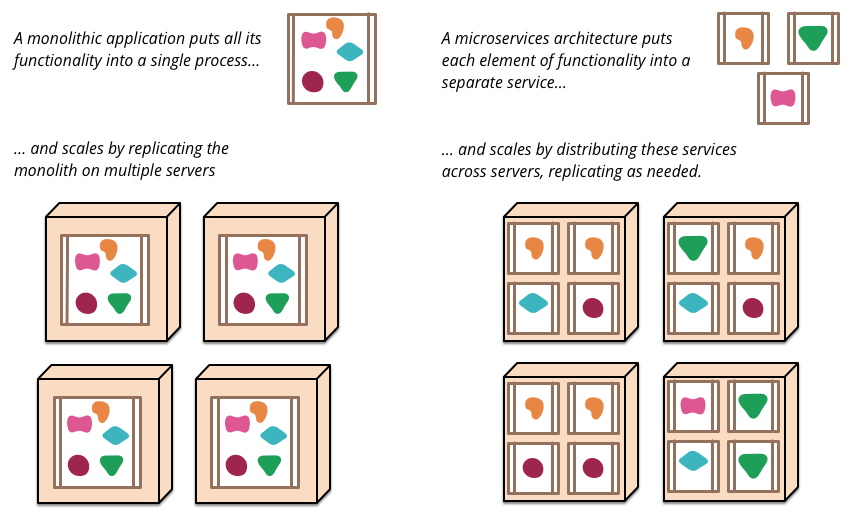
\includegraphics[width=0.6\textwidth]{images/microservices_vs_monolith.png}
\caption{Comparaison entre une architecture monolithique et microservices.}
\label{fig:archi}
\end{figure}

\subsection{Définition et caractéristiques}
Les microservices sont définis dans \cite{lewis_fowler_2014} comme « une approche visant à développer une application unique sous la forme d'une suite de petits services, chacun s'exécutant dans son propre processus et communiquant par des mécanismes légers, souvent une API de ressources HTTP. » Autrement dit, les architectures microservices reposent sur le découpage d'une application en plusieurs services autonomes, déployables indépendamment, qui communiquent généralement via des API REST ou des messages asynchrones. Ce paradigme contraste avec les architectures monolithiques, où toutes les fonctionnalités sont intégrées dans un seul bloc logiciel.

Les caractéristiques des microservices incluent :

\begin{itemize}
  \item \textbf{Autonomie :} Chaque microservice est un module indépendant qui peut être développé, déployé et mis à jour sans affecter le reste de l'application.
  \item \textbf{Scalabilité :} Les microservices permettent une scalabilité horizontale, facilitant le déploiement de plusieurs instances d'un service spécifique pour gérer une charge accrue.
  \item \textbf{Communication via API :} Les microservices communiquent principalement via des API REST ou des messages asynchrones, assurant ainsi l'interopérabilité entre différents services.
  \item \textbf{Technologies variées :} Chaque service peut être développé avec des langages et des technologies différents, permettant aux équipes de choisir les outils les plus adaptés à leurs besoins.
  \item \textbf{Résilience :} La défaillance d'un microservice n'affecte pas nécessairement l'ensemble de l'application ce qui améliore ainsi la résilience globale du système.
  \item \textbf{Développement agile :} Les équipes peuvent travailler en parallèle sur différents services, accélérant le cycle de développement et favorisant une approche DevOps.
  \item \textbf{Gestion simplifiée des versions :} Les mises à jour et les déploiements peuvent être effectués sur des services individuels sans nécessiter un arrêt complet de l'application.
\end{itemize}

\subsection{Représentation Architecturale}

La figure~\ref{fig:rep_archi} nous donne une illustration globale d'une architecture microservice \cite{mohamed_yousffi_archi}.

\begin{figure}[H]
\centering
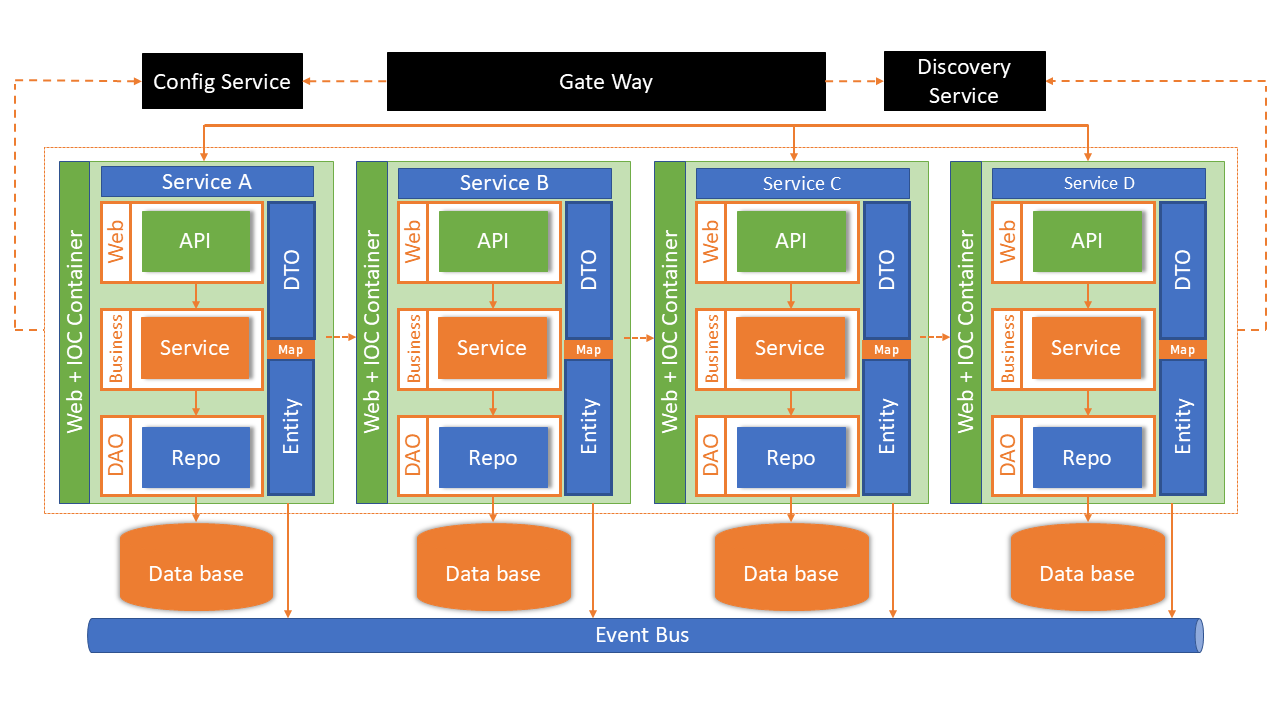
\includegraphics[width=0.6\textwidth]{images/representaton_architecturale_ms.png}
\caption{Description simplifié d'une architecture microservice.}
\label{fig:rep_archi}
\end{figure}

\subsection{Challenges et défis des microservices}

L'adoption d'une architecture microservices qui se révèle comme étant celle devant pallier aux problèmes rencontrés dans l'architecture monolithique présente des avantages significatifs tant sur la résilience, la scalabilité et l'indépendance technologique. Par ailleurs, cette approche fait face à un certain nombre de défis et de challanges. Pour bien appréhender le fonctionnement et la structuration d'une architecture microservices, il est donc essentiel de reconnaître son importance, ses bénéfices, mais aussi sa complexité. Cette compréhension permet de mieux se pencher sur les défis et les enjeux associés, qui doivent être pris en compte pour faciliter la mise en œuvre de telles architectures. Ces défis peuvent être classés en quatre catégories \cite{_defis_bares_garriga_2020, _defis_wizenty_sorgalla_rademacher_sachweh_2017}:

\textbf{Défis de conception :} Cela inclut l'identification et le dimensionnement des microservices, la définition des contrats d'échange entre eux, ainsi que l'établissement des politiques de sécurité au sein du système.

\textbf{Défis d'implémentation :} Ils portent sur la maîtrise des protocoles de communication, la gestion de la persistance des données, le choix des formats d'échange de données et l'utilisation des technologies de programmation.

\textbf{Défis opérationnels :} Ils concernent la gestion des technologies d'infrastructure, le déploiement, l'orchestration et la gestion des ressources consommées.

\textbf{Défis en matière de surveillance :} Les systèmes génèrent un grand volume de journaux non structurés et les outils opérationels de DevOps toujours ne sont pas capables de détecter avec précision les problèmes qui pourraient survenir durant la mise en service et le fonctionnement de ces applications.

\section{Surveillance et monitoring dans les systèmes distribués}

La supervision des applications distribuées implique la collecte de métriques système (CPU, RAM, latence), d’indicateurs métier (nombre de requêtes, taux d’erreurs), de traces d’exécution et de logs applicatifs. Dans le contexte des architectures microservices, où les services sont souvent interconnectés, un monitoring efficace est essentiel pour garantir la disponibilité et la performance des applications.\\

Historiquement, les outils de supervision comme Nagios, Zabbix ou Prometheus reposent sur des seuils définis manuellement. Ces approches sont efficaces pour des alertes basiques mais présentent plusieurs limites notables :
\begin{itemize}
\item Elles déclenchent des faux positifs fréquents, ce qui peut entraîner une surcharge de travail pour les équipes DevOps.
\item Elles ne tiennent pas compte des contextes d'exécution, rendant difficile la détection d'anomalies dans des environnements dynamiques.
\item Elles ne permettent pas d’anticiper des pannes complexes, ce qui peut avoir des conséquences graves sur la continuité de service.
\end{itemize}

Giamattei et al. (2024) \cite{giamattei2024} soulignent que la fragmentation de l'écosystème des outils de monitoring rend la sélection d'un outil adapté particulièrement difficile, chaque outil ayant ses propres caractéristiques, objectifs et métriques surveillées. Cela met en lumière la nécessité de choisir des outils qui non seulement surveillent des métriques de base, mais qui intègrent également des capacités avancées comme le traçage distribué pour une meilleure compréhension du comportement des microservices.

\section{Détection d’anomalies : généralités}

\subsection{Définitions et enjeux de la détection d’anomalies}

La détection d’anomalies consiste à \cite{muruti2023_detectio_anomalies_generalite} identifier des observations inhabituelles, potentiellement symptomatiques d’erreurs, d’attaques ou de défaillances système.  
Les principales catégories d’anomalies sont :

\begin{itemize}
  \item \textbf{Anomalies ponctuelles} : des observations isolées qui s’écartent fortement de comportements typiques.
  \item \textbf{Anomalies contextuelles} : des comportements observés dans un contexte particulier (temps, localisation) deviennent anormaux.
  \item \textbf{Anomalies collectives} : plusieurs observations cohérentes (ex. séries) forment un motif inhabituel global malgré la normalité individuelle.
\end{itemize}

La détection précoce des anomalies permet d’anticiper des incidents, de déclencher des actions correctives rapides, et de maintenir les niveaux de service (SLA) — un enjeu crucial dans les environnements distribués et critiques.

\subsection{Approches de détection d’anomalies}
Plusieurs approches sont sont generalement utilisees dans les systemes pour la detection d'anomalies avec chacune ayant des avantages et des limites.
\paragraph{Approches classiques}  
Des méthodes simples reposent sur des seuils statiques ou des règles métiers (e.g., alerte si la latence dépasse un seuil fixé). Bien qu’efficaces dans certains contextes, elles sont généralement insuffisantes face à la complexité et aux évolutions dynamiques des systèmes modernes.

\paragraph{Approches par apprentissage automatique}  
Elles permettent de modéliser les comportements normaux ou anormaux à partir des données.

\begin{itemize}
  \item \textbf{Supervisées} (nécessitent des labels) : exemples classiques — MLP, arbres de décision, SVM classiques.
  \item \textbf{Non supervisées} (apprenent à partir des seules données « normales ») :
    \begin{itemize}
      \item \emph{Autoencodeur} : entraîné en reconstruction ; les anomalies se détectent via une erreur élevée.
      \item \emph{Clustering} : les points isolés dans les clusters sont considérés comme anomalies.
      \item \emph{One-Class SVM} : encadre la zone des exemples normaux, hors de laquelle toute observation est potentiellement anormale.
      \item \emph{Isolation Forest} : se fonde sur la facilité d’isoler des anomalies à partir de partitions aléatoires.
    \end{itemize}
  \item \textbf{Approches hybrides} : combinaisons de modèles (e.g., autoencodeur + classifieur) pour extraire des représentations latentes robustes et les exploiter dans une phase discriminative.
\end{itemize}

\begin{figure}[H]
\centering
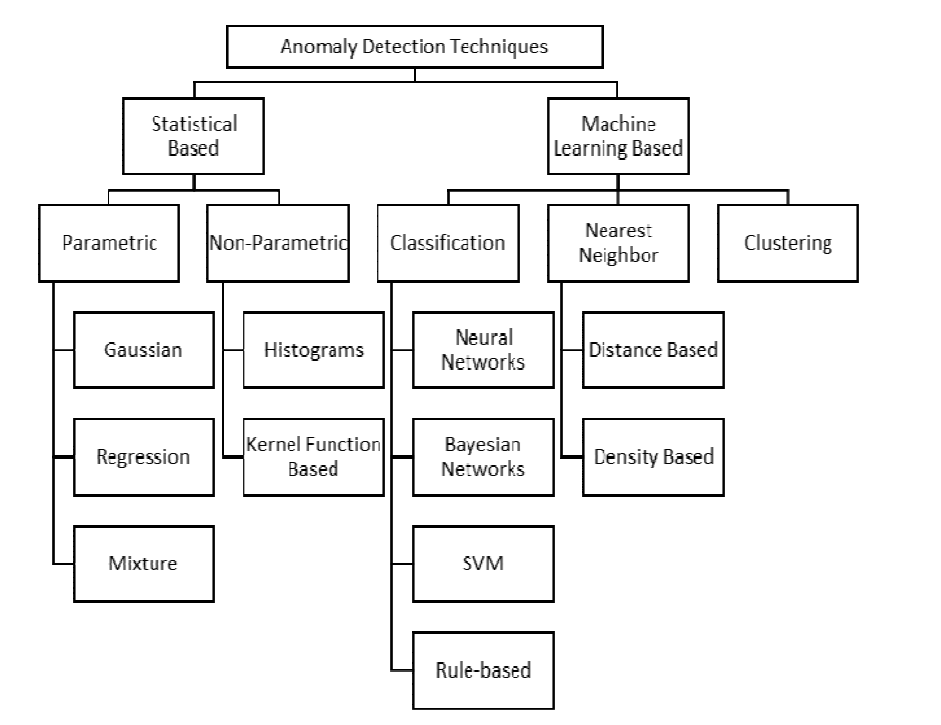
\includegraphics[width=0.8\textwidth]{images/anomalies_detections_technics.png}
\caption{Cartographie des techniques de détections d'anomalies \cite{muruti2023_detectio_anomalies_generalite}.}
\label{fig:anomalies_cartografic}
\end{figure}

Ces méthodes permettent d’adapter la détection aux volumes de données, au type d’anomalies visées, et à la disponibilité des données labellisées.

\subsection{Évaluation des performances : métriques essentielles}

L’évaluation des performances d’un modèle de détection d’anomalies ne peut se limiter à une seule mesure comme l’Accuracy, car un jeu de données déséquilibré (avec beaucoup plus d’exemples normaux que d’anomalies) pourrait conduire à une évaluation biaisée.  
Pour cela, plusieurs métriques complémentaires sont utilisées afin d’obtenir une vision complète des forces et faiblesses du modèle.

Une évaluation complète repose sur les notions suivantes \cite{nobre2023}:

\subsubsection{Matrice de confusion}

La matrice de confusion est un tableau $2 \times 2$ qui résume les prédictions du modèle :
\begin{itemize}
    \item \textbf{TP (True Positives)} : anomalies correctement détectées comme anomalies.
    \item \textbf{TN (True Negatives)} : points normaux correctement détectés comme normaux.
    \item \textbf{FP (False Positives)} : points normaux classés à tort comme anomalies (faux alarmes).
    \item \textbf{FN (False Negatives)} : anomalies non détectées, classées comme normales.
\end{itemize}

\subsubsection{Accuracy}

L’\textbf{accuracy} mesure la proportion de prédictions correctes sur l’ensemble des données :
\[
\text{\textit{Accuracy}} = \frac{TP + TN}{TP + TN + FP + FN}
\]
Elle est intuitive mais peut être trompeuse dans le cas d’un fort déséquilibre de classes.  
\textit{Exemple} : si 95\% des données sont normales, un modèle qui prédit toujours « normal » aura une accuracy de 95\%, mais sera inutile pour détecter les anomalies.

\subsubsection{Précision (Precision)}

La \textbf{précision} indique, parmi les instances prédites comme anomalies, la proportion réellement correcte :
\[
\text{\textit{Precision}} = \frac{TP}{TP + FP}
\]
Une précision élevée signifie que le modèle génère peu de fausses alertes, ce qui est important dans des contextes où le coût d’une fausse alarme est élevé (ex. alertes systèmes, cybersécurité).

\subsubsection{Rappel (Recall ou Sensibilité)}

Le \textbf{recall} mesure la capacité du modèle à détecter toutes les anomalies présentes dans les données :
\[
\text{\textit{Recall}} = \frac{TP}{TP + FN}
\]
Un rappel élevé est crucial dans les applications où manquer une anomalie peut avoir des conséquences graves (ex. panne critique, détection de fraude).

\subsubsection{F1-score}

Le \textbf{F1-score} est la moyenne harmonique entre la précision et le rappel :
\[
\textit{F1} = 2 \times \frac{\text{Precision} \times \text{Recall}}{\text{Precision} + \text{Recall}}
\]
Il équilibre les deux métriques et est particulièrement utile lorsque les classes sont déséquilibrées.  
Un F1-score élevé indique que le modèle maintient à la fois une bonne précision et un bon rappel.

En résumé, l’utilisation combinée de ces métriques permet de mieux comprendre le comportement du modèle et de choisir le compromis optimal entre précision et rappel, en fonction des contraintes du domaine d’application.


\section{Détection d’anomalies dans les systèmes à microservices}

\subsection{Spécificités des architectures microservices}

Les microservices sont des composants logiciels faiblement couplés, autonomes, et déployés indépendamment. Chaque service exécute une fonction métier précise et communique avec les autres via des API ou des messages asynchrones. Cette modularité améliore la scalabilité et la résilience, mais complexifie la surveillance et la détection d’anomalies \cite{giamattei2024}.

\paragraph{Défis spécifiques à la détection d’anomalies dans les microservices :}
\begin{itemize}
    \item \textbf{Grande hétérogénéité des métriques} : temps de réponse, taux d’erreur HTTP (2xx, 4xx, 5xx), charge CPU/mémoire, latence réseau \cite{nobre2023}.
    \item \textbf{Variabilité dynamique} : un service peut changer de comportement en fonction de la charge ou des mises à jour.
    \item \textbf{Effets de propagation} : une anomalie dans un service peut se répercuter sur d’autres, créant des cascades de dégradations \cite{chen2020robust}.
    \item \textbf{Granularité multi-niveaux} : détection possible au niveau service, application, ou infrastructure.
\end{itemize}

\subsection{Types d’anomalies observées dans les microservices}

Selon Nobre et al. (2023) \cite{nobre2023}, on retrouve :
\begin{itemize}
    \item \textbf{Anomalies de performance} : latence excessive, dégradation du throughput.
    \item \textbf{Anomalies de disponibilité} : service indisponible ou erreurs HTTP fréquentes (5xx).
    \item \textbf{Anomalies de communication} : délais réseau, timeouts, pertes de messages.
    \item \textbf{Anomalies de ressources} : consommation CPU/mémoire anormale, saturation d’I/O.
\end{itemize}

Ces anomalies peuvent être ponctuelles, contextuelles ou collectives, et nécessitent une approche multi-source pour être correctement détectées.

\subsection{Méthodes appliquées dans le contexte microservices}

Les approches suivantes sont les plus couramment employées \cite{muruti2023_detectio_anomalies_generalite, nobre2023, behera2023_model_of_anomalie}:

\paragraph{Approches supervisées}
Utilisées lorsque des logs ou métriques étiquetés sont disponibles.  
Exemples : MLP, régression logistique, forêts aléatoires.  
Limites : coût élevé d’annotation et risque de sur-apprentissage à des contextes passés.

\paragraph{Approches non supervisées}
Très utilisées car il est rare de disposer de labels.  
Exemples : Autoencodeurs LSTM pour séquences temporelles \cite{silva2022_auto_encodeur}, One-Class SVM, Isolation Forest.  
Avantages : détection d’anomalies inédites, adaptabilité.  
Limites : choix du seuil critique, sensibilité au bruit.

\paragraph{Approches hybrides}
Combinaison d’encodeurs non supervisés (réduction de dimension et extraction de caractéristiques) et de classifieurs supervisés pour une meilleure précision.  
Exemple : LSTM autoencodeur + SVM linéaire pour classifier les représentations latentes.


\section{Travaux connexes}

Plusieurs travaux de recherche récents ont proposé des approches innovantes pour la détection d’anomalies dans les systèmes microservices, en s’appuyant sur différents types de données et techniques d’apprentissage automatique.

\begin{itemize}
\item Grambow et al. (2020) ont exploré l’utilisation d’un autoencodeur LSTM pour détecter des anomalies à partir des métriques de services dans des architectures Kubernetes. Leur étude a montré la pertinence des modèles séquentiels dans la capture des dépendances temporelles au sein des services.

\item Bogatinovski et al. (2020) ont proposé une méthode d’apprentissage auto-supervisée basée sur les traces distribuées. Leur approche encode les séquences d’appels de services pour construire une représentation latente, utilisée ensuite pour identifier les anomalies sans supervision explicite.

\item Waseem et al. (2020) se sont focalisés sur la détection d’anomalies à partir de journaux d’exécution (logs) en adoptant une architecture neuronale séquentielle. Leurs travaux soulignent la richesse informationnelle des logs pour comprendre les déviations du comportement système.

\item Nobre et al. (2023) ont réalisé une étude approfondie sur les défis de la détection d’anomalies dans les architectures microservices. Leur travail met en avant l’efficacité du Perceptron Multi-Couche (MLP) pour la détection au niveau service, en montrant des scores F1 élevés sur des jeux de données injectés de fautes. Ils insistent sur la nécessité de disposer de jeux de données réalistes pour mieux entraîner les modèles.

\item Silva et al. (2022) ont développé un système de détection d’anomalies en exploitant des autoencodeurs dans un environnement Kubernetes. En utilisant des outils comme eBPF pour collecter des métriques noyau fines, ils ont montré que les autoencodeurs peuvent détecter efficacement les anomalies dans des contextes dynamiques à forte volumétrie.

\item Raeiszadeh et al. (2023) ont introduit une approche de détection en temps réel des anomalies à partir des traces distribuées dans les systèmes cloud à base de microservices. Leur modèle repose sur l’encodage des séquences de services et l’analyse en ligne des écarts de comportement, avec une attention particulière portée à la latence de détection.

\end{itemize}

Chacune de ces approches souligne l’importance d’adapter la méthode de détection aux types de données disponibles (logs, métriques, traces), aux contraintes du système (temps réel, volumétrie, distribution) et aux objectifs visés (performance, sécurité, fiabilité).

\subsection*{Tableau comparatif des travaux connexes}
\begin{table}[H]
\centering
\caption{Comparaison des approches de détection d’anomalies dans les systèmes microservices}
\label{tab:comparaison_travaux_connexes}
\begin{tabular}{|p{3.2cm}|p{2.8cm}|p{3cm}|p{3.4cm}|p{3.4cm}|}
\hline
\textbf{Référence} & \textbf{Type de données} & \textbf{Technique} & \textbf{Forces} & \textbf{Limites} \\
\hline
Grambow et al. (2020) & Métriques système & Autoencodeur LSTM & Capture les dépendances temporelles & Sensible au choix du seuil \\
\hline
Bogatinovski et al. (2020) & Traces distribuées & Auto-supervision, encodeur & Pas besoin d’étiquettes ; généralisation élevée & Entraînement coûteux, complexité de traitement \\
\hline
Waseem et al. (2020) & Logs non structurés & Réseaux séquentiels (RNN) & Exploite la richesse des logs & Prétraitement des logs complexe \\
\hline
Nobre et al. (2023) & Métriques injectées & MLP & Simplicité, bon F1 sur jeux synthétiques & Faible résilience au bruit temporel \\
\hline
Silva et al. (2022) & Métriques noyau & Autoencodeur & Haute sensibilité, approche eBPF efficace & Difficulté de généralisation à d'autres plateformes \\
\hline
Raeiszadeh et al. (2023) & Traces distribuées & Apprentissage en ligne & Détection temps réel, bon rappel & Complexité de mise en œuvre \\
\hline
\end{tabular}
\end{table}

\section*{Conclusion de l’état de l’art}

La détection d’anomalies dans les microservices nécessite des techniques adaptatives capables de traiter des données hétérogènes et séquentielles. Les modèles tels que les autoencodeurs LSTM permettent de tirer parti des relations temporelles, tandis que des modèles plus simples comme les MLP peuvent être tout aussi efficaces lorsque les signaux sont bien marqués. Ce mémoire vise à évaluer cette tension entre complexité et efficacité.


% ===========================
% METHODOLOGIE
% ===========================
\chapter{Méthodologie}

Ce chapitre présente la démarche méthodologique suivie pour la mise en œuvre et l’évaluation des modèles de détection d’anomalies utilisés dans un contexte microservices. Il détaille successivement le jeu de données exploité, les étapes de prétraitement, l’environnement d’expérimentation, la configuration des modèles testés ainsi que la méthode d’évaluation adoptée.

\section{Présentation du jeu de données}

Les expérimentations menées dans ce mémoire s’appuient sur un jeu de données issu des travaux de João Nobre et al. (2023) \cite{nobre2023}, spécialement conçu pour la détection d’anomalies dans des environnements microservices.  
L’intérêt de ce jeu de données réside dans sa conception contrôlée, qui permet :
\begin{itemize}
    \item d’introduire volontairement différents types d’anomalies au niveau des services ou de l’application ;
    \item de disposer d’un étiquetage fiable, sans incertitude sur la nature des anomalies ;
    \item de garantir la reproductibilité expérimentale et la comparaison objective de modèles.
\end{itemize}

\subsection*{Structure et niveaux d’analyse}

Le jeu de données présente deux niveaux de granularité :
\begin{itemize}
    \item \textbf{Niveau service} : chaque ligne correspond aux mesures d’un service microservices à un instant donné. Les principales colonnes sont :
    \begin{itemize}
        \item \texttt{Mean} : temps de réponse moyen ;
        \item \texttt{50th quantile} : médiane des temps de réponse (performance typique) ;
        \item \texttt{99th quantile} : temps de réponse élevé (pire cas observé) ;
        \item \texttt{2xx} : nombre de réponses HTTP réussies ;
        \item \texttt{4xx} / \texttt{5xx} : nombre de réponses HTTP en erreur (client ou serveur).
    \end{itemize}
    \item \textbf{Niveau application} : données agrégées de plusieurs services, donnant une vision globale du système.
\end{itemize}

\subsection*{Processus de génération et de collecte}

L’environnement de collecte mis en place par \cite{nobre2023} comprend :
\begin{itemize}
    \item un \textbf{cluster Kubernetes} hébergeant des microservices simulant un système applicatif complet ;
    \item un outil de surveillance (\textit{Prometheus}) collectant les métriques toutes les 15 secondes ;
    \item un mécanisme d’injection d’anomalies :
    \begin{itemize}
        \item augmentation artificielle de la latence ;
        \item génération d’erreurs HTTP (4xx, 5xx) ;
        \item arrêt ou indisponibilité de services.
    \end{itemize}
\end{itemize}

Les anomalies sont injectées de manière isolée ou combinée, ce qui permet d’obtenir un jeu de données représentatif de scénarios réels tout en restant scientifiquement maîtrisé.

\begin{figure}[H]
\centering
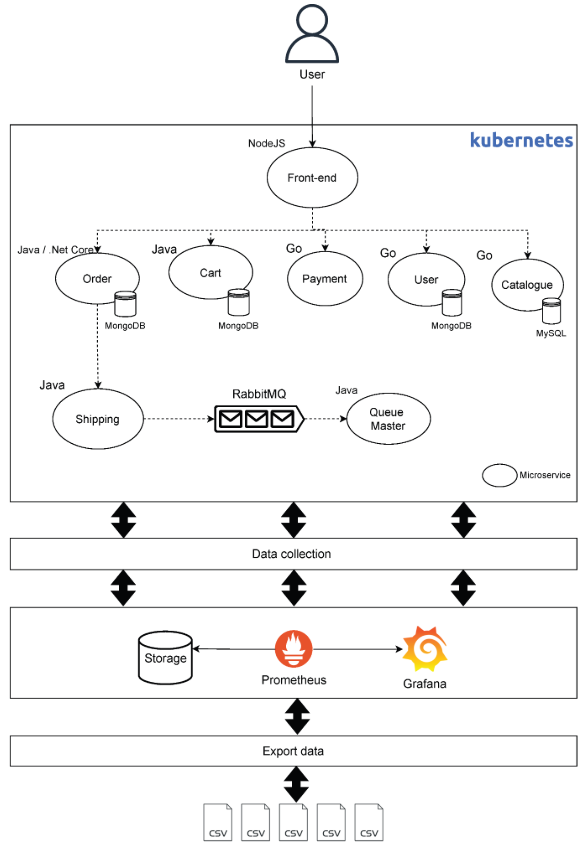
\includegraphics[width=0.50\textwidth]{images/general_architure.png}
\caption{Architecture fonctionnelle de mise en oeuvre}
\label{fig:app_achitecture}
\end{figure}


\subsection*{Étiquetage des données}

Chaque observation est associée à une variable binaire \texttt{IsError} :
\[
y =
\begin{cases}
0, & \text{comportement normal} \\
1, & \text{comportement anormal}
\end{cases}
\]
Les données se présentent sous la forme :
\[
X \in \mathbb{R}^{n \times p}, \quad y \in \{0,1\}^n
\]
où $n$ est le nombre d’observations et $p$ le nombre de variables.

\begin{figure}[H]
\centering
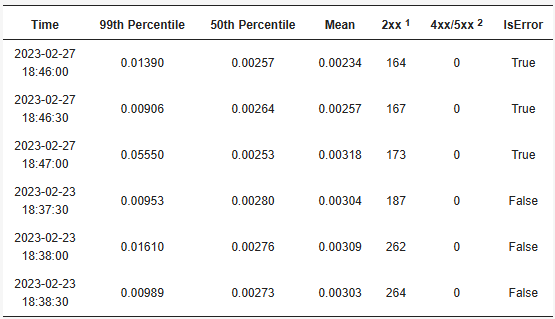
\includegraphics[width=0.75\textwidth]{images/dataset_schema.png}
\caption{Structure des colonnes principales du jeu de données aux niveaux service et application.}
\label{fig:dataset}
\end{figure}

\section{Prétraitement des données}

La qualité du prétraitement influence directement les performances des modèles. Les étapes appliquées sont les suivantes.

\subsection*{Nettoyage et préparation}
\begin{itemize}
    \item \textbf{Conversion des timestamps} : transformation des horodatages en format temporel exploitable pour l’indexation et la synchronisation.
    \item \textbf{Harmonisation des types de données} : conversion explicite des colonnes numériques et catégorielles.
    \item \textbf{Gestion des valeurs manquantes} :
    \begin{itemize}
        \item suppression lorsque l’impact sur l’information est faible ;
        \item imputation (moyenne, médiane, interpolation) lorsque la donnée est essentielle.
    \end{itemize}
\end{itemize}

\subsection*{Normalisation}
Les variables ayant des échelles différentes (par ex. temps en ms vs. taux d’erreur en \%) ont été normalisées avec un \textit{Min-Max Scaling} :
\[
x_{\text{scaled}} = \frac{x - \min(x)}{\max(x) - \min(x)}
\]
Cela garantit que toutes les variables contribuent de manière équilibrée à l’apprentissage.

% \subsection*{Gestion du déséquilibre des classes}
% Le jeu de données présente un déséquilibre modéré (plus de cas normaux que d’anomalies). Trois stratégies ont été explorées :
% \begin{itemize}
%     \item \textbf{Sous-échantillonnage} de la classe majoritaire ;
%     \item \textbf{Sur-échantillonnage} ou génération synthétique (SMOTE) de la classe minoritaire ;
%     \item \textbf{Pondération des classes} dans la fonction de perte :
%     \[
%     w_c = \frac{n_{\text{samples}}}{n_{\text{classes}} \times n_c}
%     \]
%     où $n_c$ est le nombre d’échantillons de la classe $c$.
% \end{itemize}

\subsection*{Séparation des ensembles}
Les données ont été divisées en :
\begin{itemize}
    \item \textbf{Entraînement} (70\%) : ajustement des paramètres du modèle ;
    \item \textbf{Test} (30\%) : évaluation finale, sans exposition préalable du modèle.
\end{itemize}

\section{Environnement d’expérimentation}

Les expérimentations ont été réalisées avec Python 3.x et les bibliothèques :
\begin{itemize}
    \item \texttt{Pandas}, \texttt{NumPy} pour la manipulation des données ;
    \item \texttt{Matplotlib}, \texttt{Seaborn} pour la visualisation ;
    \item \texttt{Scikit-learn} pour le MLP, le prétraitement et les métriques ;
    \item \texttt{TensorFlow/Keras} pour les modèles LSTM et hybrides.
\end{itemize}

\subsection*{Configuration matérielle}
\begin{itemize}
    \item Intel Core i7 (10\textsuperscript{e} génération) ;
    \item 32 Go RAM ;
    \item GPU NVIDIA 12 Go.
\end{itemize}


\section{Description des modèles et configurations}

Dans le cadre de ce travail, plusieurs approches d’apprentissage automatique ont été retenues pour répondre au problème de détection d’anomalies dans des systèmes à architecture microservices.  
Ces modèles ont été choisis afin de couvrir à la fois des techniques \textit{classiques} supervisées, des méthodes \textit{non supervisées} adaptées aux séries temporelles, ainsi que des architectures hybrides combinant plusieurs paradigmes d’apprentissage.

\subsection{Perceptron Multicouche (MLP)}

Le Perceptron Multicouche (\textit{Multi-Layer Perceptron}, MLP) est l’un des réseaux de neurones les plus utilisés pour des tâches de classification binaire. Dans ce travail, l’implémentation \texttt{MLPClassifier} de la bibliothèque \texttt{scikit-learn} a été retenue en raison de sa simplicité, de sa rapidité d’entraînement et de sa capacité à traiter des données tabulaires de dimension modérée.

Le MLP est un réseau \textit{feedforward}(lors de la propagation des données à travers le réseau, l'information ne circule que dans une seule direction : de l'entrée à la sortie.) composé :
\begin{itemize}
    \item \textbf{d’une couche d’entrée} recevant les variables explicatives prétraitées ;
    \item \textbf{de plusieurs couches cachées} (ici, entre 16 et 64 neurones) avec des fonctions d’activation non linéaires comme \texttt{ReLU} ou \texttt{tanh} pour capturer les relations complexes entre variables ;
    \item \textbf{d’une couche de sortie} constituée d’un seul neurone activé par une fonction \texttt{sigmoïde}, produisant une probabilité d’appartenance à la classe \texttt{anomalie}.
\end{itemize}

L’optimisation a été effectuée avec les solveurs \texttt{adam} (adaptatif, rapide à converger) et \texttt{lbfgs} (plus stable sur petits ensembles), en utilisant une recherche d’hyperparamètres (\texttt{GridSearchCV}) pour ajuster le nombre de couches, le taux d’apprentissage et la régularisation.

En raison du déséquilibre entre classes (normales vs anomalies), l’argument \texttt{class weight='balanced'} a été activé, ce qui permet au modèle de compenser automatiquement la sous-représentation des anomalies dans la fonction de perte.

\subsection{Autoencodeur LSTM}

L’autoencodeur LSTM (\textit{Long Short-Term Memory Autoencoder}) a été développé avec \texttt{Keras/TensorFlow} afin de tirer parti de la nature séquentielle des données issues de microservices. Ce modèle est non supervisé et repose sur le principe suivant :
\begin{enumerate}
    \item L’\textbf{encodeur} LSTM apprend une représentation latente compacte de la séquence d’entrée, en capturant les dépendances temporelles.
    \item Le \textbf{décodeur} LSTM reconstruit la séquence initiale à partir de cette représentation.
    \item L’\textbf{erreur de reconstruction} est utilisée comme indicateur d’anomalie : si elle dépasse un seuil empirique (déterminé sur un ensemble de validation), l’observation est considérée comme anormale.
\end{enumerate}

La configuration retenue inclut 32 à 64 unités LSTM par couche, des fonctions d’activation \texttt{tanh}, et une perte \texttt{MSE} (\textit{Mean Squared Error}) pour mesurer la qualité de reconstruction.  
L’entraînement a été réalisé exclusivement sur des séquences normales, sur 20 à 50 époques, avec une taille de lot (\textit{batch size}) de 16 et l’optimiseur \texttt{Adam}.  
Cette méthode est particulièrement adaptée aux systèmes microservices où les anomalies se traduisent souvent par des ruptures dans les tendances temporelles.

\subsection{Modèle Hybride MLP + LSTM}

Le modèle hybride combine deux sous-architectures :
\begin{itemize}
    \item une branche LSTM dédiée à l’analyse des variables séquentielles (métriques temporelles collectées dans le temps) ;
    \item une branche dense (MLP) pour traiter les variables statiques ou dérivées qui ne possèdent pas de structure temporelle.
\end{itemize}

Les sorties des deux branches sont concaténées, puis transmises à une couche dense finale activée par une fonction \texttt{sigmoïde}.  
L’entraînement s’effectue sur 18 à 50 époques, avec un \texttt{dropout} compris entre 0,2 et 0,5 pour limiter le surapprentissage.  
Ce type d’architecture permet de capturer simultanément :
\begin{itemize}
    \item les dynamiques temporelles (via LSTM) ;
    \item les relations instantanées ou dérivées (via MLP).
\end{itemize}
Cette combinaison est particulièrement pertinente dans le contexte microservices, où certaines anomalies apparaissent dans l’évolution des métriques, tandis que d’autres sont visibles dans l’état global du système à un instant donné.

\section{Méthodes d’évaluation}

L’évaluation des modèles est une étape cruciale afin de mesurer leur capacité à distinguer efficacement les comportements normaux des anomalies. Dans ce travail, plusieurs métriques complémentaires ont été retenues :

\begin{itemize}
    \item \textbf{Accuracy} : proportion globale de prédictions correctes, mais qui peut être trompeuse en cas de classes déséquilibrées.
    \item \textbf{Precision} : capacité du modèle à éviter les fausses alertes, calculée comme la proportion d’alertes réellement justifiées.
    \item \textbf{Recall (Sensibilité)} : capacité à détecter toutes les anomalies, même au prix de quelques fausses alertes.
    \item \textbf{F1-score} : moyenne harmonique entre précision et rappel, offrant un compromis adapté lorsque les deux sont importants.
\end{itemize}

En complément, des visualisations ont été utilisées pour interpréter et comparer les performances :
\begin{itemize}
    \item \textbf{Matrices de confusion} : pour visualiser la répartition des prédictions vraies/fausses par classe.
    \item \textbf{Courbes de perte et d’accuracy} : pour suivre la convergence du modèle durant l’entraînement.
    \item \textbf{Distribution des erreurs de reconstruction} : dans le cas des LSTM autoencodeurs, pour évaluer la séparation entre séquences normales et anormales.
\end{itemize}

Ces outils permettent non seulement d’évaluer quantitativement les modèles, mais également d’identifier leurs forces et limites dans différents scénarios de détection.


\section*{Conclusion}

Cette méthodologie fournit un cadre reproductible allant of the preparation of data for the implementation and evaluation of models, guaranteeing an équitable comparison of the approaches.



% ===========================
% RESULTATS ET DISCUSSIONS
% ===========================
\chapter{Résultats et discussions}

Ce chapitre présente les résultats expérimentaux obtenus pour chaque modèle testé, aux niveaux \textit{service} et \textit{application}. Les résultats sont accompagnés d’une analyse critique, visant à interpréter les performances observées, à mettre en lumière les forces et les limites de chaque approche, et à proposer des pistes d’amélioration.

\section{Résultats expérimentaux}

Les modèles ont été évalués selon des métriques standards de classification : \textit{accuracy}, \textit{precision}, \textit{recall} et \textit{F1-score}. Les matrices de confusion permettent de visualiser les proportions de vrais positifs (VP), vrais négatifs (VN), faux positifs (FP) et faux négatifs (FN), tandis que les courbes de perte et d’apprentissage offrent un aperçu de la convergence des entraînements et des risques de surapprentissage. L'analyse des courbes est essentielle pour interpréter la stabilité de l'apprentissage, la vitesse de convergence et la capacité du modèle à généraliser.

\subsection{Perceptron Multicouche (MLP)}

\subsubsection*{Niveau service}

Le MLP a été entraîné avec deux couches cachées de tailles $(16, 8)$ et une fonction d’activation \texttt{tanh}.  
L’optimisation des hyperparamètres a été effectuée via \texttt{GridSearchCV} afin de sélectionner la configuration maximisant la performance globale.

\begin{itemize}
    \item Accuracy = 0.97
    \item Precision = 0.97
    \item Recall = 0.98
    \item F1-score = 0.97
\end{itemize}

\begin{figure}[H]
    \centering
    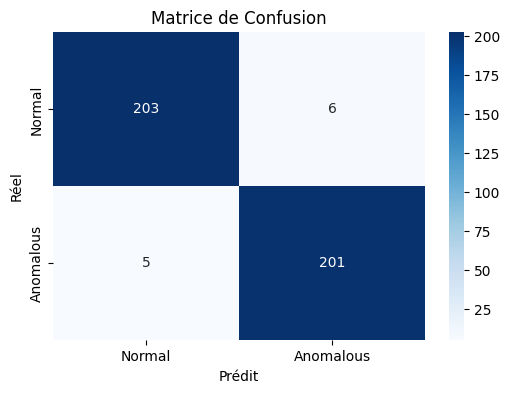
\includegraphics[width=0.65\textwidth]{images/confusion_matrix_mlp_service.png}
    \caption{Matrice de confusion du MLP – niveau service.}
\end{figure}

\paragraph{Analyse des métriques :}
Le taux d’\textit{accuracy} très élevé (97\%) confirme que le modèle classe correctement la quasi-totalité des instances, tandis que la précision et le rappel équilibrés (97\% et 98\%) montrent qu’il est à la fois efficace pour identifier les anomalies et prudent pour éviter les fausses alertes. Le faible nombre de FP et FN visible dans la matrice de confusion traduit une robustesse sur ce type de données.

\paragraph{Analyse de la courbe de perte :}
\begin{figure}[H]
    \centering
    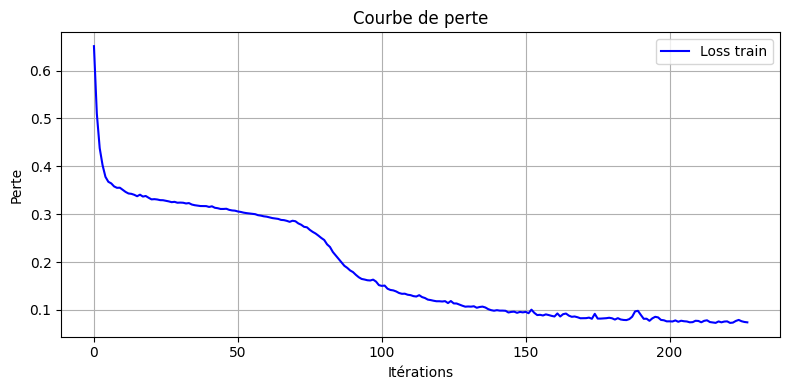
\includegraphics[width=0.75\textwidth]{images/loss_curve_mlp_service.png}
    \caption{Courbe de perte du MLP – niveau service.}
\end{figure}

La courbe présente trois phases distinctes :
\begin{enumerate}
    \item \textbf{Phase initiale (0–30 itérations)} : La perte diminue rapidement, passant d'environ 0.68 à 0.60. Cette décroissance abrupte indique que le modèle apprend rapidement des motifs discriminants clairs et stables dès les premières itérations.
    \item \textbf{Phase intermédiaire (30–120 itérations)} : La perte continue de décroître de manière régulière et stable, ce qui montre que le modèle affine progressivement ses poids pour optimiser la séparation entre classes. L’absence d’oscillations marquées traduit un apprentissage stable et une absence de surajustement précoce.
    \item \textbf{Phase de stabilisation (120–220 itérations)} : La perte converge vers une valeur proche de 0.52, signe que le modèle atteint un plateau de performance où de nouvelles itérations n'apportent plus d’amélioration significative.
\end{enumerate}
Cette dynamique illustre un entraînement maîtrisé, où la richesse des signaux au niveau service permet au MLP d’apprendre efficacement sans surapprentissage marqué.

\subsubsection*{Niveau application}

Pour ce niveau, la configuration retenue est composée de deux couches cachées $(8, 16)$ avec activation \texttt{tanh}.

\begin{itemize}
    \item Accuracy = 0.52
    \item Precision = 0.62
    \item Recall = 0.12
    \item F1-score = 0.20
\end{itemize}

\begin{figure}[H]
    \centering
    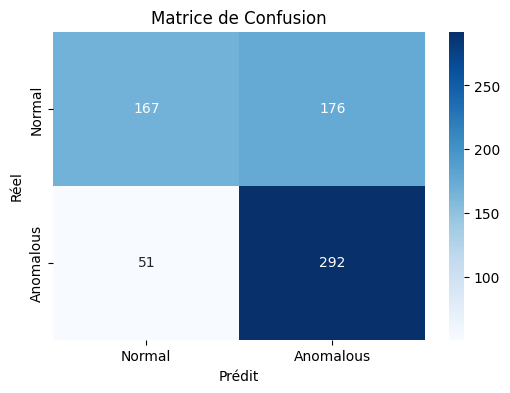
\includegraphics[width=0.75\textwidth]{images/confusion_matrix_mlp_application.png}
    \caption{Matrice de confusion – MLP niveau application.}
\end{figure}

\paragraph{Analyse des métriques :}
Le contraste avec le niveau service est frappant : un \textit{recall} très faible (12\%) indique que le modèle ne parvient pas à détecter la majorité des anomalies. Malgré une précision de 62\% (donc relativement correcte sur les anomalies identifiées), l’efficacité globale est limitée, ce que reflète un F1-score faible (0.20). La matrice de confusion montre un grand nombre de faux négatifs, ce qui est problématique dans un contexte de détection d’anomalies.

\begin{figure}[H]
    \centering
    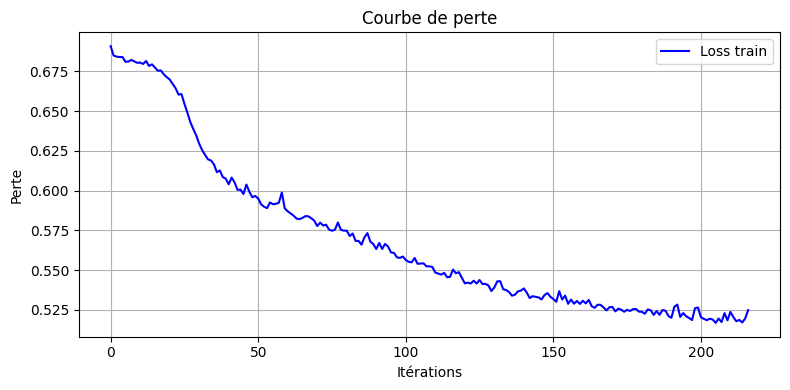
\includegraphics[width=0.75\textwidth]{images/loss_curve_mlp_application.png}
    \caption{Courbe de perte – MLP niveau application.}
\end{figure}


\paragraph{Analyse de la courbe de perte :}
La dynamique d’apprentissage diffère fortement :
\begin{enumerate}
    \item \textbf{Phase initiale (0–10 itérations)} : La perte démarre à un niveau très élevé (~0.63) mais chute immédiatement vers 0.35, traduisant un ajustement rapide des poids sur des motifs facilement capturables.
    \item \textbf{Phase intermédiaire (10–80 itérations)} : La perte diminue plus lentement, oscillant légèrement, signe que le modèle peine à extraire des motifs discriminants supplémentaires.
    \item \textbf{Phase tardive (80–220 itérations)} : Une longue phase de convergence progressive, avec une perte finale très basse (~0.07). Cependant, cette faible perte ne se traduit pas par de bonnes performances en test, ce qui indique un possible surajustement aux données d’entraînement.
\end{enumerate}
Ce décalage entre une perte faible et de faibles scores en test reflète une réalité courante : en l’absence de signaux discriminants nets, le modèle « apprend par cœur » les données d’entraînement, perdant en capacité de généralisation.

\paragraph{Interprétation générale :}
La comparaison des courbes et métriques pour les deux niveaux met en évidence que :
\begin{itemize}
    \item Au niveau service, la richesse des signaux et la stabilité des patterns permettent au MLP d'apprendre efficacement et de généraliser.
    \item Au niveau application, les signaux faibles et la variabilité rendent l’apprentissage plus fragile, menant à un ajustement qui ne se traduit pas par de bonnes performances en détection réelle.
\end{itemize}


\subsection{Autoencodeur LSTM}

L’autoencodeur LSTM a été conçu pour apprendre uniquement la structure des données normales.  
En phase d’inférence, les observations présentant une erreur de reconstruction supérieure à un seuil prédéfini sont considérées comme des anomalies.  
Cette approche est particulièrement adaptée aux séries temporelles, car les couches LSTM capturent les dépendances temporelles et les dynamiques séquentielles.

\subsubsection*{Niveau service}

Entraîné uniquement sur données normales et évalué via l’erreur de reconstruction :

\begin{itemize}
    \item Accuracy = 0.85
    \item Precision = 0.78
    \item Recall = 0.95
    \item F1-score = 0.86
\end{itemize}

\begin{figure}[H]
    \centering
    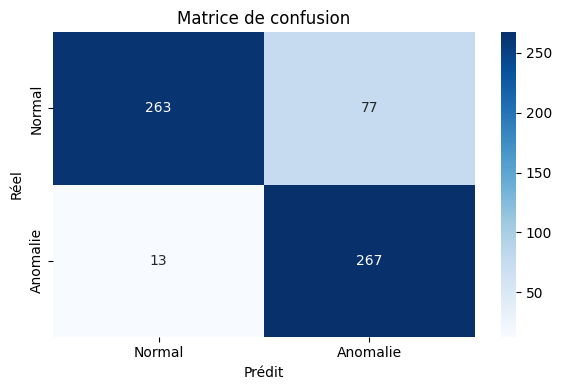
\includegraphics[width=0.48\textwidth]{images/confusion_matrix_lstm_service.png}
    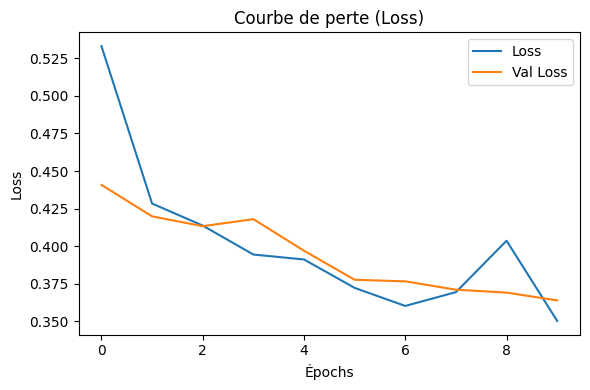
\includegraphics[width=0.48\textwidth]{images/loss_curve_lstm_service.png}
    \caption{Matrice de confusion et courbe de perte – LSTM autoencodeur niveau service.}
\end{figure}

\paragraph{Analyse des métriques :}
La matrice de confusion montre que sur un total de 550 échantillons normaux, 263 ont été correctement classés et 77 ont été faussement signalés comme anomalies.  
Pour les anomalies, 267 sur 280 ont été détectées correctement, ce qui explique le \textbf{rappel élevé (95\%)}.  
Cette sensibilité élevée réduit considérablement le risque de laisser passer une anomalie.  
En revanche, la précision de 0.78 traduit encore 22\% de faux positifs, souvent liés à des fluctuations naturelles de service interprétées comme anomalies.

\paragraph{Analyse de la courbe de perte :}
La courbe de perte présente un profil d’apprentissage stable :
\begin{enumerate}
    \item \textbf{Phase initiale (0--2 époques)} : forte baisse de la perte (de $\approx 0.69$ à $\approx 0.67$) montrant que le modèle capture rapidement les structures temporelles majeures.
    \item \textbf{Phase intermédiaire (3--6 époques)} : décroissance plus lente, indiquant l’ajustement progressif sur des motifs plus subtils.
    \item \textbf{Phase finale (7--9 époques)} : la perte atteint $\approx 0.63$ avec une courbe de validation parallèle, signe d’une convergence sans surapprentissage notable.
\end{enumerate}

\paragraph{Interprétation :}
La combinaison d’un rappel élevé et d’une précision modérée traduit un compromis fréquent en détection d’anomalies : maximiser la détection au prix d’un surplus de fausses alertes.  
Ce choix est souvent privilégié dans un contexte de supervision critique.

\subsubsection*{Niveau application}

\begin{itemize}
    \item Accuracy = 0.58
    \item Precision = 0.64
    \item Recall = 0.35
    \item F1-score = 0.45
\end{itemize}

\begin{figure}[H]
    \centering
    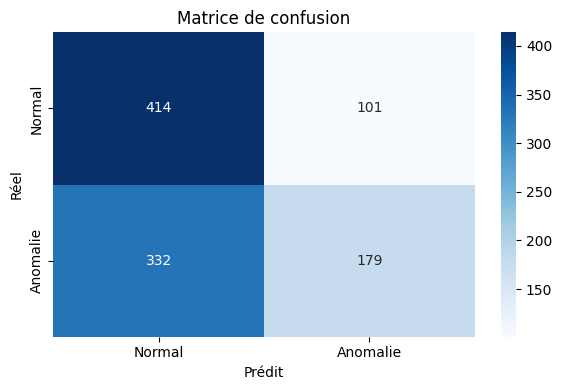
\includegraphics[width=0.48\textwidth]{images/confusion_matrix_lstm_application.png}
    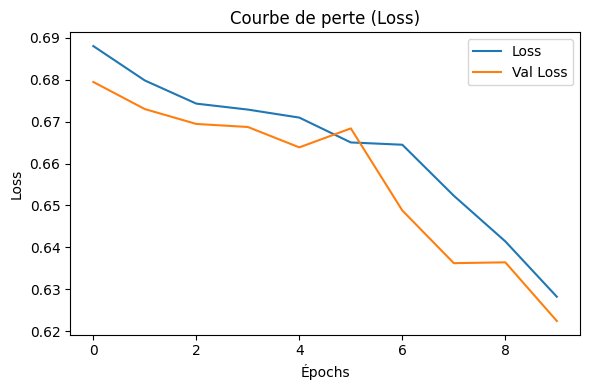
\includegraphics[width=0.48\textwidth]{images/loss_curve_lstm_application.png}
    \caption{Résultats du LSTM autoencodeur – niveau application.}
\end{figure}

\paragraph{Analyse des métriques :}
La matrice de confusion révèle que sur 515 échantillons normaux, 414 sont correctement classés mais 101 sont faussement détectés comme anomalies.  
En revanche, sur 511 anomalies réelles, seules 179 sont détectées, laissant 332 faux négatifs, ce qui explique le \textbf{rappel faible (35\%)}.  
Ce résultat illustre la difficulté du modèle à distinguer les anomalies des fluctuations normales au niveau applicatif.

\paragraph{Analyse de la courbe de perte :}
Le profil de perte diffère nettement du niveau service :
\begin{enumerate}
    \item \textbf{Phase initiale (0--1 époque)} : perte passant rapidement de $\approx 0.53$ à $\approx 0.43$.
    \item \textbf{Phase intermédiaire (2--6 époques)} : poursuite de la baisse mais avec des fluctuations, signe d’une difficulté à stabiliser l’apprentissage.
    \item \textbf{Phase finale (7--9 époques)} : convergence vers $\approx 0.35$, mais sans amélioration notable en rappel, suggérant un surajustement sur les données d’entraînement.
\end{enumerate}

\paragraph{Interprétation :}
Les signaux applicatifs étant moins corrélés dans le temps et plus bruités, l’autoencodeur LSTM perd son avantage structurel.  
La modélisation séquentielle ne suffit pas à extraire des motifs discriminants, ce qui se traduit par une forte proportion d’anomalies non détectées.


\subsection{Modèle hybride LSTM + MLP}

Le modèle hybride vise à combiner deux paradigmes complémentaires :
\begin{itemize}
    \item \textbf{LSTM} : exploite les dépendances temporelles pour analyser les variations séquentielles et contextuelles des métriques.
    \item \textbf{MLP} : traite efficacement les variables indépendantes ou faiblement corrélées dans un cadre non-séquentiel, permettant d’intégrer des signaux plus statiques.
\end{itemize}

La logique sous-jacente est que les métriques issues d’un environnement microservices contiennent à la fois des patterns dynamiques (latence, throughput) et des informations plus stables (répartition des codes HTTP, moyennes glissantes). En combinant ces deux approches, le modèle cherche à capturer simultanément la dimension temporelle et la dimension statique.

\subsubsection*{Niveau service}

\begin{figure}[H]
    \centering
    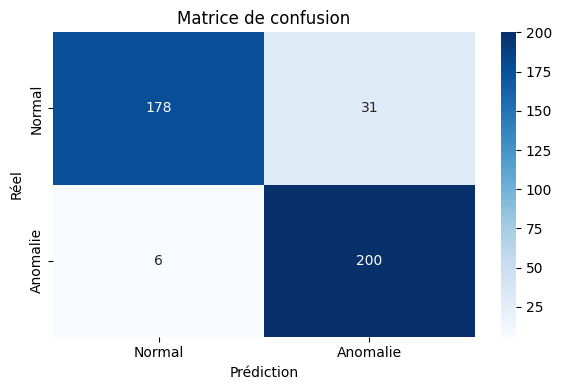
\includegraphics[width=0.48\textwidth]{images/confusion_matrix_hybrid_service.png}
    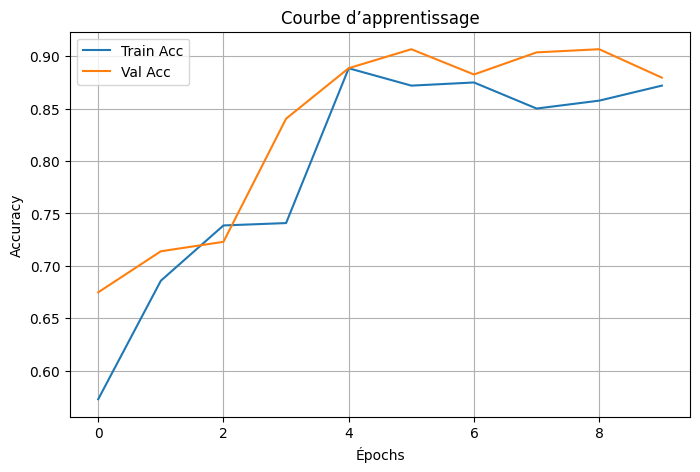
\includegraphics[width=0.48\textwidth]{images/loss_curve_hybrid_service.png}
    \caption{Matrice de confusion et courbe d’apprentissage – Modèle hybride, niveau service.}
\end{figure}

\paragraph{Performances globales :}
\begin{itemize}
    \item Accuracy = 0.91
    \item Precision = 0.87
    \item Recall = 0.97
    \item F1-score = 0.92
\end{itemize}

\paragraph{Analyse de la matrice de confusion :}
La matrice de confusion montre que :
\begin{itemize}
    \item Les anomalies sont détectées presque intégralement (rappel de 97\%), confirmant la capacité du LSTM à identifier les ruptures temporelles.
    \item Le nombre de faux positifs est plus bas que dans le LSTM pur, ce qui indique que l’ajout du MLP aide à filtrer certaines fluctuations normales considérées à tort comme des anomalies.
\end{itemize}

\paragraph{Analyse de la courbe d’apprentissage :}
La courbe d’accuracy montre :
\begin{enumerate}
    \item Une montée rapide en performance dès les premières époques, signe que les motifs dominants sont rapidement identifiés.
    \item Une convergence stable au-delà de l’époque 4, avec peu d’écart entre accuracy d’entraînement et de validation, ce qui suggère un faible surapprentissage.
    \item L’écart de performance réduit par rapport au LSTM seul vient probablement de la capacité du MLP à mieux généraliser sur des variations mineures.
\end{enumerate}

\paragraph{Interprétation :}
Ce niveau de performance s’explique par le fait qu’au niveau service, les signaux sont relativement stables et bien structurés. Le LSTM capte la dynamique, tandis que le MLP stabilise la décision finale. On obtient ainsi un compromis optimal entre \textit{sensibilité} et \textit{spécificité}, réduisant le volume de fausses alertes sans perdre de véritables anomalies.

\subsubsection*{Niveau application}

\begin{figure}[H]
    \centering
    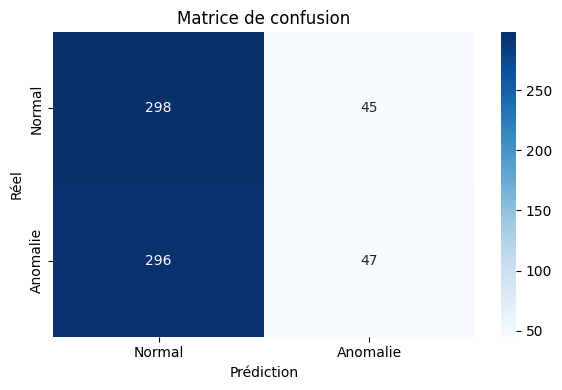
\includegraphics[width=0.48\textwidth]{images/confusion_matrix_hybrid_application.png}
    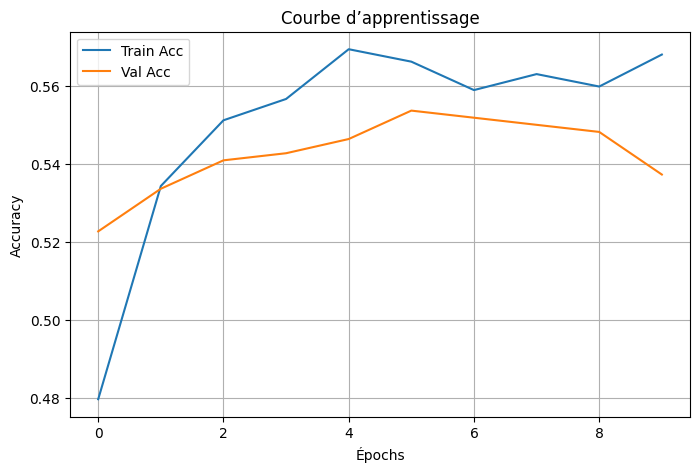
\includegraphics[width=0.48\textwidth]{images/loss_curve_hybrid_application.png}
    \caption{Matrice de confusion et courbe d’apprentissage – Modèle hybride, niveau application.}
\end{figure}

\paragraph{Performances globales :}
\begin{itemize}
    \item Accuracy = 0.50
    \item Precision = 0.51
    \item Recall = 0.14
    \item F1-score = 0.22
\end{itemize}

\paragraph{Analyse de la matrice de confusion :}
Ici, la détection des anomalies se dégrade fortement :
\begin{itemize}
    \item Le rappel chute à 14\%, ce qui signifie que la majorité des anomalies passent inaperçues.
    \item Le taux de faux négatifs est particulièrement élevé, confirmant que les anomalies au niveau agrégé sont plus difficiles à distinguer des comportements normaux.
\end{itemize}

\paragraph{Analyse de la courbe d’apprentissage :}
La courbe montre :
\begin{enumerate}
    \item Une progression lente de l’accuracy, traduisant la difficulté à trouver des motifs discriminants.
    \item Un plateau prématuré, signe que le modèle atteint rapidement sa limite d’apprentissage.
    \item Une faible marge entre l’entraînement et la validation, ce qui suggère que la limite vient plus de la nature des données que d’un manque de capacité du modèle.
\end{enumerate}

\paragraph{Interprétation :}
Au niveau application, les données sont le résultat d’agrégations qui diluent les signaux temporels et masquent les anomalies locales. La composante LSTM perd donc une grande partie de sa pertinence, et le MLP, privé de variables distinctives, ne parvient pas à compenser. En d’autres termes, le modèle hybride ne peut pas « inventer » des signaux discriminants inexistants dans les données, même s’il est performant en conditions favorables.\\

En résumé, le modèle hybride excelle au niveau service grâce à la complémentarité LSTM–MLP, mais n’apporte qu’un gain marginal, voire nul, au niveau application, faute de signaux exploitables. Cette observation confirme l’importance de la granularité des données pour tirer parti d’architectures complexes : un modèle avancé ne peut surperformer que si les données contiennent l’information nécessaire à la discrimination.


\subsection{Résumé comparatif et tendances}

\begin{table}[H]
\centering
\caption{Résumé comparatif des performances des modèles sur les deux niveaux d'analyse.}
\begin{tabular}{|c|c|c|c|c|c|}
\hline
\textbf{Modèle} & \textbf{Niveau} & \textbf{Accuracy} & \textbf{Precision} & \textbf{Recall} & \textbf{F1-score} \\
\hline
MLP & Service & 0.97 & 0.97 & 0.98 & 0.97 \\
MLP & Application & 0.52 & 0.62 & 0.12 & 0.20 \\
LSTM & Service & 0.85 & 0.78 & 0.95 & 0.86 \\
LSTM & Application & 0.58 & 0.64 & 0.35 & 0.45 \\
Hybride & Service & 0.91 & 0.87 & 0.97 & 0.92 \\
Hybride & Application & 0.50 & 0.51 & 0.14 & 0.22 \\
\hline
\end{tabular}
\end{table}

\paragraph{Observation générale :}
Trois tendances structurantes se dégagent de l'analyse :
\begin{enumerate}
    \item \textbf{Supériorité systématique des performances au niveau service} :  
    Les trois modèles obtiennent des scores nettement plus élevés lorsqu'ils sont appliqués sur les données désagrégées par service. Cette différence s’explique par la richesse des signaux capturés à ce niveau : latences spécifiques, variations locales de charge, distribution fine des codes HTTP.  
    En revanche, au niveau application, l’agrégation des métriques dilue ces signaux et atténue les ruptures temporelles, ce qui rend la tâche de détection plus complexe. Les modèles doivent alors inférer des anomalies à partir de motifs beaucoup moins distinctifs.

    \item \textbf{Limitation du LSTM par la granularité des données} :  
    Le LSTM excelle dans la modélisation de séries temporelles lorsqu'il existe une structure séquentielle forte. Au niveau service, cette condition est remplie, et le modèle atteint un rappel élevé (95\%), détectant presque toutes les anomalies.  
    Cependant, lorsque les données sont agrégées au niveau application, les patterns temporels deviennent moins marqués, entraînant une chute significative du rappel (35\%). Autrement dit, la valeur ajoutée du LSTM est directement proportionnelle à la clarté des dépendances temporelles dans les données d’entrée.

    \item \textbf{Rendement conditionnel des modèles hybrides} :  
    La combinaison LSTM + MLP offre un compromis solide au niveau service (F1-score = 0.92) grâce à la complémentarité entre :
    \begin{itemize}
        \item le LSTM, qui capture les dynamiques temporelles ;
        \item le MLP, qui filtre les variations normales et améliore la précision.
    \end{itemize}
    En revanche, au niveau application, cette combinaison ne parvient pas à compenser le manque de signaux discriminants. Les performances restent proches, voire inférieures, à celles des modèles individuels. Cela illustre un principe clé : un modèle complexe ne surperforme que si les données contiennent des informations distinctives exploitables.
\end{enumerate}

\paragraph{Lecture stratégique des résultats :}
\begin{itemize}
    \item Pour un déploiement opérationnel où la granularité des métriques est fine (niveau service), le \textbf{MLP} reste la solution la plus efficace en précision globale, tandis que le \textbf{LSTM} et l’hybride sont préférés si la sensibilité aux anomalies (rappel élevé) est prioritaire.
    \item Dans des contextes où seules des métriques agrégées au niveau application sont disponibles, les performances sont limitées quelle que soit l’architecture utilisée. L’enjeu devient alors moins un choix de modèle qu’une optimisation de la collecte de données pour augmenter la qualité du signal.
    \item Ces résultats rappellent l’importance de l’alignement entre la nature des données et la conception du modèle : la sophistication algorithmique n’apporte un gain que si elle répond à une structure exploitable dans les données.
\end{itemize}



\section{Discussion}

Les résultats obtenus mettent en évidence un contraste très marqué entre les performances observées au \textbf{niveau service} et celles au \textbf{niveau application}. Cette différence, bien que prévisible, mérite une analyse approfondie afin d’identifier les causes sous-jacentes et de comprendre leurs implications dans un contexte opérationnel.

\subsection*{Analyse par niveau}

\paragraph{Au niveau service.}
Les données issues du niveau service présentent des motifs temporels et statistiques plus nets, avec une variabilité moins importante et des indicateurs directement liés à la santé de chaque composant (temps de réponse moyen, distribution des latences, taux de codes \texttt{2xx} ou \texttt{4xx/5xx}).  
Ces indicateurs, lorsqu’ils sont altérés, traduisent souvent un problème technique localisé, ce qui facilite la tâche des modèles.  
Ainsi :
\begin{itemize}
    \item Le \textbf{MLP} parvient à modéliser efficacement les relations non linéaires entre les indicateurs grâce à sa structure dense, sans avoir besoin de capturer des dépendances temporelles complexes.
    \item L’\textbf{autoencodeur LSTM} excelle dans la capture des motifs séquentiels, ce qui améliore la détection d’anomalies évolutives ou progressives. Son rappel très élevé montre qu’il détecte presque toutes les anomalies, même subtiles.
    \item Le \textbf{modèle hybride} combine ces forces, atteignant un équilibre entre rappel et précision, et réduisant le risque de faux positifs.
\end{itemize}
Globalement, le niveau service bénéficie de signaux discriminants forts, stables et directement observables, ce qui explique des \textit{accuracy} supérieures à 90\% pour la plupart des approches.

\paragraph{Au niveau application.}
À l’inverse, le niveau application agrège les métriques issues de plusieurs services. Cette agrégation dilue souvent les signaux propres à un service particulier et introduit un bruit statistique important. Par exemple, une dégradation localisée dans un microservice peut être masquée par la stabilité des autres, ce qui rend l’anomalie difficile à détecter.  
Conséquences :
\begin{itemize}
    \item Le \textbf{MLP} peine à trouver des frontières de décision claires, ce qui se traduit par un rappel extrêmement faible (12\%).
    \item L’\textbf{autoencodeur LSTM} capture certains motifs temporels globaux, mais l’absence de signaux forts limite son efficacité, le rappel restant modeste.
    \item Le \textbf{modèle hybride} n’apporte pas d’amélioration notable, confirmant que le problème ne réside pas uniquement dans le type de modèle, mais dans la nature même des données agrégées.
\end{itemize}
Ces résultats illustrent que la granularité de la donnée joue un rôle déterminant dans la détection d’anomalies et que l’agrégation excessive peut réduire significativement la sensibilité des modèles.

\subsection*{Forces et limites des approches}

\begin{itemize}
    \item \textbf{MLP} :
    \begin{itemize}
        \item \textit{Forces} : simplicité d’implémentation, rapidité d’entraînement, robustesse sur des jeux de données avec des signaux forts et peu de dépendances temporelles.
        \item \textit{Limites} : faible capacité à capturer des dépendances séquentielles ou des anomalies évolutives ; performances dégradées en contexte bruité.
    \end{itemize}
    \item \textbf{Autoencodeur LSTM} :
    \begin{itemize}
        \item \textit{Forces} : excellente détection des anomalies subtiles grâce à la modélisation des séquences temporelles ; rappel élevé utile dans des environnements critiques où les faux négatifs sont coûteux.
        \item \textit{Limites} : sensibilité élevée au choix du seuil d’erreur de reconstruction ; plus grand risque de faux positifs ; entraînement plus coûteux.
    \end{itemize}
    \item \textbf{Hybride LSTM + MLP} :
    \begin{itemize}
        \item \textit{Forces} : capacité à traiter à la fois des variables temporelles et statiques ; bonne performance lorsque les signaux sont variés.
        \item \textit{Limites} : complexité plus importante, ce qui ne garantit pas un gain de performance lorsque les données ne contiennent pas d’informations discriminantes suffisantes.
    \end{itemize}
\end{itemize}

\subsection*{Implications pratiques}

Les différences observées suggèrent qu’en production :
\begin{itemize}
    \item La surveillance au niveau service est plus fiable pour détecter rapidement des incidents localisés.
    \item La surveillance au niveau application, bien que moins précise, reste utile pour détecter des pannes globales ou des tendances de dégradation à long terme.
    \item Les équipes d’exploitation devraient combiner les deux niveaux d’analyse pour maximiser la couverture et la réactivité.
\end{itemize}

\section*{Conclusion}
Les résultats révèlent un écart net entre les performances au \textbf{niveau service} et au \textbf{niveau application}.
Au niveau service, la richesse des signaux permet au MLP, au LSTM et au modèle hybride d’atteindre d’excellents scores :
le MLP maximise la précision, le LSTM le rappel, et l’hybride trouve un équilibre entre les deux.
Au niveau application, l’agrégation des métriques dilue les signaux, entraînant une forte baisse des performances pour tous les modèles, y compris les plus sophistiqués.

Deux enseignements se dégagent :
\begin{enumerate}
\item La granularité des données conditionne directement la qualité de la détection.
\item La complexité du modèle n’est utile que si les données contiennent suffisamment d’information exploitable.
\end{enumerate}

En pratique, il est recommandé de privilégier la surveillance fine au niveau service, complétée par une vision globale au niveau application, et de choisir le modèle selon l’objectif prioritaire : précision ou rappel.



% ===========================
% CONCLUSION
% ===========================
\chapter{Conclusion}

Ce mémoire avait pour objectif d’explorer et de comparer plusieurs approches d’apprentissage automatique appliquées à la détection d’anomalies dans des environnements microservices, un domaine où la surveillance proactive est devenue un enjeu stratégique. Les architectures microservices, bien qu’offrant flexibilité et scalabilité, introduisent une complexité importante dans le suivi des performances et la détection précoce de dysfonctionnements.  

Trois modèles représentatifs ont été implémentés et évalués :
\begin{itemize}
    \item \textbf{Le perceptron multicouche (MLP)} — un modèle simple et rapide, particulièrement efficace lorsque les signaux discriminants sont bien marqués.
    \item \textbf{L’autoencodeur LSTM} — adapté aux données séquentielles et performant sur les séries temporelles présentant des motifs temporels forts.
    \item \textbf{Le modèle hybride LSTM + MLP} — combinant la capture des dépendances temporelles avec le traitement efficace de variables statiques.
\end{itemize}

Les résultats expérimentaux, obtenus sur deux niveaux d’agrégation des données (service et application), mettent en évidence plusieurs points essentiels :
\begin{itemize}
    \item \textbf{Supériorité du niveau service} : Les performances sont systématiquement plus élevées au niveau service, avec des F1-scores atteignant jusqu’à 0.97 pour le MLP. Ce niveau bénéficie de signaux plus nets, moins dilués par l’agrégation.
    \item \textbf{Limites du niveau application} : L’agrégation des métriques entraîne une perte de granularité et une dilution des signaux d’anomalie, réduisant fortement le rappel (jusqu’à 0.12 pour le MLP et 0.14 pour l’hybride).
    \item \textbf{Apport conditionnel de la complexité} : Le LSTM et le modèle hybride montrent un réel intérêt uniquement lorsque les données présentent à la fois des patterns temporels marqués et des signaux statiques exploitables.
\end{itemize}

\section*{Apports du travail}
Ce travail apporte plusieurs contributions notables :
\begin{itemize}
    \item Une \textbf{analyse comparative approfondie} de trois architectures de détection d’anomalies dans un contexte microservices, avec des mesures détaillées (accuracy, précision, rappel, F1-score) et une discussion nuancée sur leurs forces et limites.
    \item La \textbf{mise en évidence de l’importance de la granularité des données} dans les performances des modèles, soulignant que la qualité et la structure des données sont souvent plus déterminantes que la sophistication algorithmique.
    \item La \textbf{production de scripts et visualisations reproductibles}, permettant de répliquer les expériences ou de les adapter à d’autres environnements DevOps.
    \item Une \textbf{première évaluation des modèles hybrides} dans ce contexte, offrant un point de départ pour de futures expérimentations plus ciblées.
\end{itemize}

\section*{Perspectives}
Les pistes d’amélioration identifiées ouvrent plusieurs directions prometteuses :
\begin{itemize}
    \item \textbf{Enrichissement des données} : intégrer des logs applicatifs, des traces distribuées et des métriques métier afin de renforcer les signaux exploités par les modèles.
    \item \textbf{Modèles avancés} : tester des architectures intégrant des mécanismes d’attention (\textit{Attention Mechanisms}) pour mieux capturer les dépendances à long terme.
    \item \textbf{Explicabilité et interprétabilité} : intégrer des méthodes comme SHAP ou LIME pour comprendre les décisions du modèle, expliquer pourquoi une anomalie est détectée, afin d’améliorer la confiance et faciliter l’adoption par les équipes de supervision(DevOps).\\
\end{itemize}

En définitive, ce travail montre que la performance d’un système de détection d’anomalies ne repose pas uniquement sur le choix d’un algorithme, mais sur un alignement optimal entre la nature des données, la granularité d’observation et la complexité du modèle. Les enseignements tirés ouvrent la voie vers des solutions plus fines, plus explicables et mieux intégrées aux pratiques DevOps modernes, afin d’assurer une surveillance proactive et fiable des architectures microservices.



% ===========================
% BIBLIOGRAPHIE
% ===========================
\bibliographystyle{apalike}
\bibliography{references}
\nocite{*}


\end{document}
